\section{Compressor Control}
\label{sec:intro:compressor}

Compressor control generally consists of two separate, sometimes competing tasks: process control and anti-surge control.
Process control seeks primarily to regulate an output variable of the compressor -- in this report, the output pressure is used, but mass flow or other variables could equally be chosen.
The manipulated variable used in process control varies depending on the type of compressor studied.
Gas turbine-driven compressors, for example, may have a valve regulating the fuel flow to the turbine, which can be adjusted by the control system to increase or decrease the compressor speed. 
For the electric, variable-speed drivers considered here, the manipulated variable is the torque applied by the driver to the compressor, which is adjusted to maintain the output pressure at the desired setpoint.

Anti-surge control keeps the compressor away from an unstable regime known as surge, which is characterized by unstable oscillations in the mass flow rate through the compressor.
Surge occurs when the load on the compressor increases, resulting in a reduced and then oscillatory mass flow.
In extreme cases (known as ``deep surge'') the mass flow can actually become negative.
Operating in the surge regime can cause serious damage to the compressor.

The conditions leading to surge are determined experimentally and plotted as a line on the compressor map, known as the surge line (SL).
\footnote{The transition to surge only collapses onto a single line in the compressor map if (quasi\babelhyphen{nobreak})invariant coordinates are used; the transition to surge is then invariant to the inlet conditions. 
For a detailed discussion of compressor maps and invariant coordinate systems, see \cite{Batson1996}.
For the purposes of this work, the pressure ratio and mass flow rate are used and are assumed to be quasi-invariant for the cases studied.}
This plot is then used to define a surge distance (\g{sd}) for the compressor, which is defined as the horizontal distance between the current operating point and the surge line.
\footnote{The surge distance is sometimes also defined as the angular distance between the operating point and the surge line.}
To avoid entering the surge regime, a surge control line (SCL) that is offset from the surge line, and a corresponding surge control distance (\g{scd}) are defined to add a safety margin for the controller.
The controller should maintain the operating point to the right of the surge control line.
A compressor map with the surge line and surge distance labeled is shown in \fig{intro:comp-map}.

\begin{figure}
  \centering
  % This file was created by matlab2tikz.
%
\definecolor{mycolor1}{rgb}{0.00000,0.44700,0.74100}%
\definecolor{mycolor2}{rgb}{0.85000,0.32500,0.09800}%
\definecolor{mycolor3}{rgb}{0.92900,0.69400,0.12500}%
\definecolor{mycolor4}{rgb}{0.49400,0.18400,0.55600}%
\definecolor{mycolor5}{rgb}{0.46600,0.67400,0.18800}%
\definecolor{mycolor6}{rgb}{0.30100,0.74500,0.93300}%
\definecolor{mycolor7}{rgb}{0.63500,0.07800,0.18400}%

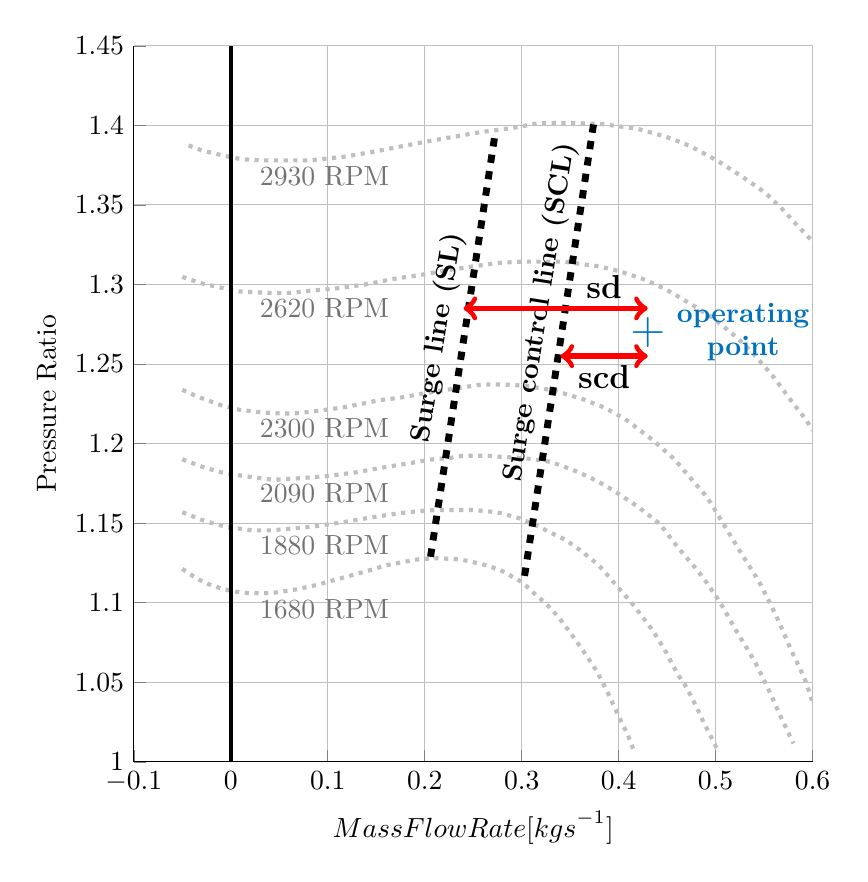
\begin{tikzpicture}

\begin{axis}[%
width=0.711\linewidth,
height=0.75\linewidth,
at={(0\linewidth,0\linewidth)},
scale only axis,
unbounded coords=jump,
xmin=-0.1,
xmax=0.6,
xlabel={$\text{Mass Flow Rate [kg s}^{\text{-1}}\text{]}$},
xmajorgrids,
ymin=1,
ymax=1.45,
ylabel={Pressure Ratio},
ymajorgrids,
axis background/.style={fill=white},
axis x line*=bottom,
axis y line*=left
]
\addplot [color=lightgray,dotted,line width=1.5pt,forget plot]
  table[row sep=crcr]{%
-0.05	1.12127525252525\\
-0.0434343434343434	1.11858101214162\\
-0.0368686868686869	1.11589173156934\\
-0.0303030303030303	1.11379621127096\\
-0.0237373737373737	1.11184596191483\\
-0.0171717171717172	1.11047434862862\\
-0.0106060606060606	1.1091027353424\\
-0.00404040404040405	1.10815605550454\\
0.00252525252525253	1.10721307137027\\
0.00909090909090909	1.1065745842261\\
0.0156565656565657	1.10615548016642\\
0.0222222222222222	1.10606060606061\\
0.0287878787878788	1.10606060606061\\
0.0353535353535354	1.10606060606061\\
0.0419191919191919	1.10606060606061\\
0.0484848484848485	1.10663090232468\\
0.0550505050505051	1.10722647125159\\
0.0616161616161616	1.1078220401785\\
0.0681818181818182	1.10845892075839\\
0.0747474747474747	1.1093464352377\\
0.0813131313131313	1.11023394971702\\
0.0878787878787879	1.11112146419633\\
0.0944444444444445	1.11217031425365\\
0.101010101010101	1.11327970735279\\
0.107575757575758	1.11438910045193\\
0.114141414141414	1.11549560206442\\
0.120707070707071	1.11659575022107\\
0.127272727272727	1.11769589837772\\
0.133838383838384	1.11879604653437\\
0.14040404040404	1.11989619469102\\
0.146969696969697	1.12107374247526\\
0.153535353535354	1.12233105465429\\
0.16010101010101	1.12354695949393\\
0.166666666666667	1.12430134680135\\
0.173232323232323	1.12505573410876\\
0.17979797979798	1.12581012141618\\
0.186363636363636	1.1265645087236\\
0.192929292929293	1.12728811685882\\
0.19949494949495	1.12753957929463\\
0.206060606060606	1.12779104173044\\
0.212626262626263	1.12802013541702\\
0.219191919191919	1.12781058338718\\
0.225757575757576	1.12760103135734\\
0.232323232323232	1.12739147932751\\
0.238888888888889	1.12690952737249\\
0.245454545454545	1.12607131925314\\
0.252020202020202	1.12523311113378\\
0.258585858585859	1.12439490301443\\
0.265151515151515	1.1231403592199\\
0.271717171717172	1.12179323902809\\
0.278282828282828	1.12044066631856\\
0.284848484848485	1.11822188012028\\
0.291414141414141	1.11600309392199\\
0.297979797979798	1.1137843077237\\
0.304545454545455	1.11064623507805\\
0.311111111111111	1.10687429854097\\
0.317676767676768	1.10332242883379\\
0.324242424242424	1.09992768595041\\
0.330808080808081	1.09588230792776\\
0.337373737373737	1.09135598408326\\
0.343939393939394	1.08630730707751\\
0.35050505050505	1.08085895430172\\
0.357070707070707	1.07525156871748\\
0.363636363636364	1.06959366391185\\
0.37020202020202	1.06365268850117\\
0.376767676767677	1.05761759004183\\
0.383333333333333	1.05011311026936\\
0.38989898989899	1.0420157564097\\
0.396464646464647	1.03339418718207\\
0.403030303030303	1.0248708677686\\
0.40959595959596	1.01667506291875\\
0.416161616161616	1.00623660850934\\
0.422727272727273	nan\\
0.429292929292929	nan\\
0.435858585858586	nan\\
0.442424242424242	nan\\
0.448989898989899	nan\\
0.455555555555556	nan\\
0.462121212121212	nan\\
0.468686868686869	nan\\
0.475252525252525	nan\\
0.481818181818182	nan\\
0.488383838383838	nan\\
0.494949494949495	nan\\
0.501515151515151	nan\\
0.508080808080808	nan\\
0.514646464646465	nan\\
0.521212121212121	nan\\
0.527777777777778	nan\\
0.534343434343434	nan\\
0.540909090909091	nan\\
0.547474747474747	nan\\
0.554040404040404	nan\\
0.560606060606061	nan\\
0.567171717171717	nan\\
0.573737373737374	nan\\
0.58030303030303	nan\\
0.586868686868687	nan\\
0.593434343434343	nan\\
0.6	nan\\
};
\addplot [color=lightgray,dotted,line width=1.5pt,forget plot]
  table[row sep=crcr]{%
-0.05	1.15691121743753\\
-0.0434343434343434	1.15532303363244\\
-0.0368686868686869	1.15373484982735\\
-0.0303030303030303	1.15214666602226\\
-0.0237373737373737	1.15084688987318\\
-0.0171717171717172	1.14973749677404\\
-0.0106060606060606	1.1486281036749\\
-0.00404040404040405	1.14762597111082\\
0.00252525252525253	1.14708712303409\\
0.00909090909090909	1.14654827495737\\
0.0156565656565657	1.14600942688064\\
0.0222222222222222	1.14547057880391\\
0.0287878787878788	1.14545454545455\\
0.0353535353535354	1.14545454545455\\
0.0419191919191919	1.14551056253826\\
0.0484848484848485	1.14586418158861\\
0.0550505050505051	1.14621780063897\\
0.0616161616161616	1.14657141968932\\
0.0681818181818182	1.14692503873967\\
0.0747474747474747	1.14727865779002\\
0.0813131313131313	1.14763227684037\\
0.0878787878787879	1.14815167996986\\
0.0944444444444445	1.14873197789864\\
0.101010101010101	1.14931227582743\\
0.107575757575758	1.14989257375621\\
0.114141414141414	1.15047287168499\\
0.120707070707071	1.15110691395127\\
0.127272727272727	1.15179272059437\\
0.133838383838384	1.15247852723748\\
0.14040404040404	1.15316433388059\\
0.146969696969697	1.15384194819003\\
0.153535353535354	1.15443751711694\\
0.16010101010101	1.15503308604385\\
0.166666666666667	1.15562865497076\\
0.173232323232323	1.15618251739018\\
0.17979797979798	1.15662627462984\\
0.186363636363636	1.1570700318695\\
0.192929292929293	1.15751378910915\\
0.19949494949495	1.15780755790226\\
0.206060606060606	1.15807698194062\\
0.212626262626263	1.15833333333333\\
0.219191919191919	1.15833333333333\\
0.225757575757576	1.15833333333333\\
0.232323232323232	1.15833333333333\\
0.238888888888889	1.15833333333333\\
0.245454545454545	1.15833333333333\\
0.252020202020202	1.15817308182839\\
0.258585858585859	1.15779588817468\\
0.265151515151515	1.15741869452097\\
0.271717171717172	1.15704150086726\\
0.278282828282828	1.15636560945162\\
0.284848484848485	1.15525621635247\\
0.291414141414141	1.15414682325333\\
0.297979797979798	1.15303743015419\\
0.304545454545455	1.15128137434956\\
0.311111111111111	1.14952113729892\\
0.317676767676768	1.14776090024827\\
0.324242424242424	1.14578924162258\\
0.330808080808081	1.14381346534124\\
0.337373737373737	1.14183768905991\\
0.343939393939394	1.13986191277858\\
0.35050505050505	1.13723503979186\\
0.357070707070707	1.13440608738904\\
0.363636363636364	1.13143447461629\\
0.37020202020202	1.12820138615593\\
0.376767676767677	1.12496829769557\\
0.383333333333333	1.12097254597255\\
0.38989898989899	1.11633016254228\\
0.396464646464647	1.11168777911202\\
0.403030303030303	1.10710322926232\\
0.40959595959596	1.10252302061014\\
0.416161616161616	1.09785991225385\\
0.422727272727273	1.09257920110193\\
0.429292929292929	1.08729848995001\\
0.435858585858586	1.0818873422007\\
0.442424242424242	1.07537217909119\\
0.448989898989899	1.06885701598167\\
0.455555555555556	1.06093674843675\\
0.462121212121212	1.05394049926878\\
0.468686868686869	1.04807304243331\\
0.475252525252525	1.04069291398837\\
0.481818181818182	1.03246097337006\\
0.488383838383838	1.02383940414243\\
0.494949494949495	1.01615651464136\\
0.501515151515151	1.00813437404347\\
0.508080808080808	nan\\
0.514646464646465	nan\\
0.521212121212121	nan\\
0.527777777777778	nan\\
0.534343434343434	nan\\
0.540909090909091	nan\\
0.547474747474747	nan\\
0.554040404040404	nan\\
0.560606060606061	nan\\
0.567171717171717	nan\\
0.573737373737374	nan\\
0.58030303030303	nan\\
0.586868686868687	nan\\
0.593434343434343	nan\\
0.6	nan\\
};
\addplot [color=lightgray,dotted,line width=1.5pt,forget plot]
  table[row sep=crcr]{%
-0.05	1.19012626262626\\
-0.0434343434343434	1.18861748801143\\
-0.0368686868686869	1.18710871339659\\
-0.0303030303030303	1.18560127793082\\
-0.0237373737373737	1.18442254776298\\
-0.0171717171717172	1.18324381759514\\
-0.0106060606060606	1.1820650874273\\
-0.00404040404040405	1.1813212087202\\
0.00252525252525253	1.18069255263068\\
0.00909090909090909	1.18006389654117\\
0.0156565656565657	1.1794552793778\\
0.0222222222222222	1.17894092439547\\
0.0287878787878788	1.17842656941314\\
0.0353535353535354	1.17791221443081\\
0.0419191919191919	1.17739785944848\\
0.0484848484848485	1.17744062730694\\
0.0550505050505051	1.17766250592677\\
0.0616161616161616	1.1778843845466\\
0.0681818181818182	1.17813360881543\\
0.0747474747474747	1.17843536373839\\
0.0813131313131313	1.17873711866136\\
0.0878787878787879	1.17903887358433\\
0.0944444444444445	1.1793406285073\\
0.101010101010101	1.17971067423547\\
0.107575757575758	1.1802250292178\\
0.114141414141414	1.18073938420013\\
0.120707070707071	1.18125373918246\\
0.127272727272727	1.18176809416479\\
0.133838383838384	1.18246668221416\\
0.14040404040404	1.18318514631646\\
0.146969696969697	1.18390361041876\\
0.153535353535354	1.18462207452106\\
0.16010101010101	1.18529775133859\\
0.166666666666667	1.18595374030157\\
0.173232323232323	1.18660972926454\\
0.17979797979798	1.18726571822751\\
0.186363636363636	1.18792233835683\\
0.192929292929293	1.18858797421632\\
0.19949494949495	1.1892536100758\\
0.206060606060606	1.18991924593529\\
0.212626262626263	1.19034041856012\\
0.219191919191919	1.19063056752451\\
0.225757575757576	1.19093656955227\\
0.232323232323232	1.19162237619538\\
0.238888888888889	1.19230818283849\\
0.245454545454545	1.19242424242424\\
0.252020202020202	1.19242424242424\\
0.258585858585859	1.19242424242424\\
0.265151515151515	1.19235648785838\\
0.271717171717172	1.19204215981362\\
0.278282828282828	1.19172783176887\\
0.284848484848485	1.1914879634131\\
0.291414141414141	1.19126608479327\\
0.297979797979798	1.19104420617344\\
0.304545454545455	1.19069837990293\\
0.311111111111111	1.1901595318262\\
0.317676767676768	1.18962068374947\\
0.324242424242424	1.18908183567275\\
0.330808080808081	1.18838217330431\\
0.337373737373737	1.18691530909544\\
0.343939393939394	1.18544844488658\\
0.35050505050505	1.18398158067771\\
0.357070707070707	1.18235099309594\\
0.363636363636364	1.1805907560453\\
0.37020202020202	1.17883051899466\\
0.376767676767677	1.17679599020508\\
0.383333333333333	1.17453282828283\\
0.38989898989899	1.17226966636058\\
0.396464646464647	1.16980556830936\\
0.403030303030303	1.16716521273339\\
0.40959595959596	1.16452485715743\\
0.416161616161616	1.16188450158147\\
0.422727272727273	1.15898473370064\\
0.429292929292929	1.15584145325307\\
0.435858585858586	1.1526981728055\\
0.442424242424242	1.14955489235792\\
0.448989898989899	1.1444300432779\\
0.455555555555556	1.13908646651702\\
0.462121212121212	1.13405121288644\\
0.468686868686869	1.12933629221508\\
0.475252525252525	1.12462137154372\\
0.481818181818182	1.11990645087236\\
0.488383838383838	1.11468544876373\\
0.494949494949495	1.1089018127402\\
0.501515151515151	1.10311817671666\\
0.508080808080808	1.09668134513176\\
0.514646464646465	1.08948037537914\\
0.521212121212121	1.08243036424855\\
0.527777777777778	1.07582947530864\\
0.534343434343434	1.06922858636874\\
0.540909090909091	1.06256574004508\\
0.547474747474747	1.0543360603278\\
0.554040404040404	1.04610638061051\\
0.560606060606061	1.03730834515959\\
0.567171717171717	1.0283928587992\\
0.573737373737374	1.01985970819304\\
0.58030303030303	1.01156144781145\\
0.586868686868687	nan\\
0.593434343434343	nan\\
0.6	nan\\
};
\addplot [color=lightgray,dotted,line width=1.5pt,forget plot]
  table[row sep=crcr]{%
-0.05	1.23375841750842\\
-0.0434343434343434	1.23199818045778\\
-0.0368686868686869	1.23023794340714\\
-0.0303030303030303	1.22865566438799\\
-0.0237373737373737	1.22718880017912\\
-0.0171717171717172	1.22572193597025\\
-0.0106060606060606	1.22425507176138\\
-0.00404040404040405	1.22324524708363\\
0.00252525252525253	1.22223939734041\\
0.00909090909090909	1.22123354759718\\
0.0156565656565657	1.22075067276298\\
0.0222222222222222	1.22027918069585\\
0.0287878787878788	1.21980768862871\\
0.0353535353535354	1.21951658312927\\
0.0419191919191919	1.2192808370957\\
0.0484848484848485	1.21904509106214\\
0.0550505050505051	1.21893939393939\\
0.0616161616161616	1.21893939393939\\
0.0681818181818182	1.21909131421164\\
0.0747474747474747	1.21953507145129\\
0.0813131313131313	1.21997882869095\\
0.0878787878787879	1.22042258593061\\
0.0944444444444445	1.22095458553792\\
0.101010101010101	1.22149343361465\\
0.107575757575758	1.22203228169137\\
0.114141414141414	1.2225711297681\\
0.120707070707071	1.2233013304036\\
0.127272727272727	1.22410960251869\\
0.133838383838384	1.22491787463378\\
0.14040404040404	1.22572614674887\\
0.146969696969697	1.22653441886396\\
0.153535353535354	1.22731353943475\\
0.16010101010101	1.22778503150189\\
0.166666666666667	1.22825652356902\\
0.173232323232323	1.22872801563616\\
0.17979797979798	1.22941512284947\\
0.186363636363636	1.23013358695177\\
0.192929292929293	1.23085205105407\\
0.19949494949495	1.23157051515637\\
0.206060606060606	1.23223012957861\\
0.212626262626263	1.23285878566813\\
0.219191919191919	1.23348744175764\\
0.225757575757576	1.23411509029691\\
0.232323232323232	1.23471860014284\\
0.238888888888889	1.23532210998878\\
0.245454545454545	1.23592561983471\\
0.252020202020202	1.23652912968064\\
0.258585858585859	1.23712121212121\\
0.265151515151515	1.23712121212121\\
0.271717171717172	1.23712121212121\\
0.278282828282828	1.23712121212121\\
0.284848484848485	1.23703163542736\\
0.291414141414141	1.23680975680753\\
0.297979797979798	1.2365878781877\\
0.304545454545455	1.23636599956787\\
0.311111111111111	1.23568513416998\\
0.317676767676768	1.23499932752688\\
0.324242424242424	1.23431352088377\\
0.330808080808081	1.23362771424066\\
0.337373737373737	1.23264833829572\\
0.343939393939394	1.23144817667028\\
0.35050505050505	1.23024801504485\\
0.357070707070707	1.22904785341941\\
0.363636363636364	1.22779398260682\\
0.37020202020202	1.22624083226802\\
0.376767676767677	1.22468768192921\\
0.383333333333333	1.22313453159041\\
0.38989898989899	1.2210902849049\\
0.396464646464647	1.21887149870661\\
0.403030303030303	1.21665271250833\\
0.40959595959596	1.21416397622206\\
0.416161616161616	1.21111050378727\\
0.422727272727273	1.20805703135249\\
0.429292929292929	1.2050035589177\\
0.435858585858586	1.20189761548942\\
0.442424242424242	1.19834755757216\\
0.448989898989899	1.1947974996549\\
0.455555555555556	1.19124744173764\\
0.462121212121212	1.18689212197735\\
0.468686868686869	1.18217720130599\\
0.475252525252525	1.17750015486758\\
0.481818181818182	1.1729199462154\\
0.488383838383838	1.16833973756322\\
0.494949494949495	1.16277714989836\\
0.501515151515151	1.15610372371736\\
0.508080808080808	1.14943029753636\\
0.514646464646465	1.14287309118117\\
0.521212121212121	1.13633506785022\\
0.527777777777778	1.12979704451927\\
0.534343434343434	1.12338988172322\\
0.540909090909091	1.1170066045066\\
0.547474747474747	1.11022453976999\\
0.554040404040404	1.10214181861909\\
0.560606060606061	1.09405909746819\\
0.567171717171717	1.08540678247118\\
0.573737373737374	1.07597694112846\\
0.58030303030303	1.06704441105268\\
0.586868686868687	1.05881473133539\\
0.593434343434343	1.04973116810238\\
0.6	1.03733766233766\\
};
\addplot [color=lightgray,dotted,line width=1.5pt,forget plot]
  table[row sep=crcr]{%
-0.05	1.30474598930481\\
-0.0434343434343434	1.30341471758584\\
-0.0368686868686869	1.30208344586687\\
-0.0303030303030303	1.30075397468446\\
-0.0237373737373737	1.29986646020514\\
-0.0171717171717172	1.29897894572583\\
-0.0106060606060606	1.29809143124651\\
-0.00404040404040405	1.29725064497792\\
0.00252525252525253	1.29644237286283\\
0.00909090909090909	1.29563410074774\\
0.0156565656565657	1.2953322949614\\
0.0222222222222222	1.29517513093902\\
0.0287878787878788	1.29501796691664\\
0.0353535353535354	1.29486080289426\\
0.0419191919191919	1.29470363887188\\
0.0484848484848485	1.29469696969697\\
0.0550505050505051	1.29469696969697\\
0.0616161616161616	1.29475804623111\\
0.0681818181818182	1.29517715029079\\
0.0747474747474747	1.29559625435046\\
0.0813131313131313	1.29601535841014\\
0.0878787878787879	1.296402699433\\
0.0944444444444445	1.29676193148415\\
0.101010101010101	1.29712116353531\\
0.107575757575758	1.29748039558646\\
0.114141414141414	1.29790423171105\\
0.120707070707071	1.29847002219161\\
0.127272727272727	1.29903581267218\\
0.133838383838384	1.29960160315274\\
0.14040404040404	1.30023249115736\\
0.146969696969697	1.30101831126926\\
0.153535353535354	1.30180413138115\\
0.16010101010101	1.30258995149304\\
0.166666666666667	1.30337577160494\\
0.173232323232323	1.30404413908202\\
0.17979797979798	1.30458298715874\\
0.186363636363636	1.30512183523547\\
0.192929292929293	1.30575822504197\\
0.19949494949495	1.30644403168508\\
0.206060606060606	1.30712983832819\\
0.212626262626263	1.30781564497129\\
0.219191919191919	1.30848744175764\\
0.225757575757576	1.30911609784716\\
0.232323232323232	1.30974475393667\\
0.238888888888889	1.31037341002619\\
0.245454545454545	1.3110020661157\\
0.252020202020202	1.31159256708499\\
0.258585858585859	1.31213141516172\\
0.265151515151515	1.31267026323845\\
0.271717171717172	1.31320911131517\\
0.278282828282828	1.31367747786209\\
0.284848484848485	1.31387600083772\\
0.291414141414141	1.31407452381336\\
0.297979797979798	1.314273046789\\
0.304545454545455	1.31439393939394\\
0.311111111111111	1.31439393939394\\
0.317676767676768	1.31439393939394\\
0.324242424242424	1.31439393939394\\
0.330808080808081	1.31439393939394\\
0.337373737373737	1.31439393939394\\
0.343939393939394	1.31430511828239\\
0.35050505050505	1.31376627020566\\
0.357070707070707	1.31322742212894\\
0.363636363636364	1.31268857405221\\
0.37020202020202	1.31214972597548\\
0.376767676767677	1.31161087789876\\
0.383333333333333	1.31085332491582\\
0.38989898989899	1.30991034078155\\
0.396464646464647	1.30896735664728\\
0.403030303030303	1.30790078818488\\
0.40959595959596	1.3065806103969\\
0.416161616161616	1.30526043260892\\
0.422727272727273	1.30394025482094\\
0.429292929292929	1.30244426589124\\
0.435858585858586	1.30055829762269\\
0.442424242424242	1.29867232935415\\
0.448989898989899	1.2967863610856\\
0.455555555555556	1.29455520113415\\
0.462121212121212	1.29217292542651\\
0.468686868686869	1.28979064971888\\
0.475252525252525	1.28740837401124\\
0.481818181818182	1.28490970309152\\
0.488383838383838	1.28239507873346\\
0.494949494949495	1.2798804543754\\
0.501515151515151	1.27677900802901\\
0.508080808080808	1.2735873694207\\
0.514646464646465	1.27032769827909\\
0.521212121212121	1.26687008978676\\
0.527777777777778	1.26341248129443\\
0.534343434343434	1.25933464839189\\
0.540909090909091	1.25512880427653\\
0.547474747474747	1.25054859562435\\
0.554040404040404	1.24596838697217\\
0.560606060606061	1.24119180015645\\
0.567171717171717	1.23574344738065\\
0.573737373737374	1.23036526885012\\
0.58030303030303	1.22508455769819\\
0.586868686868687	1.21990698228072\\
0.593434343434343	1.2148777335646\\
0.6	1.20833333333333\\
};
\addplot [color=lightgray,dotted,line width=1.5pt,forget plot]
  table[row sep=crcr]{%
-0.05	nan\\
-0.0434343434343434	1.38740536679931\\
-0.0368686868686869	1.38589659218447\\
-0.0303030303030303	1.38438781756964\\
-0.0237373737373737	1.38333349275584\\
-0.0171717171717172	1.38239050862157\\
-0.0106060606060606	1.3814475244873\\
-0.00404040404040405	1.38058397831125\\
0.00252525252525253	1.37977570619616\\
0.00909090909090909	1.37896743408107\\
0.0156565656565657	1.37859227799884\\
0.0222222222222222	1.37834081556304\\
0.0287878787878788	1.37808935312723\\
0.0353535353535354	1.3780303030303\\
0.0419191919191919	1.3780303030303\\
0.0484848484848485	1.3780303030303\\
0.0550505050505051	1.3780303030303\\
0.0616161616161616	1.3780303030303\\
0.0681818181818182	1.3780303030303\\
0.0747474747474747	1.3780303030303\\
0.0813131313131313	1.3780303030303\\
0.0878787878787879	1.37842099445635\\
0.0944444444444445	1.37884009851602\\
0.101010101010101	1.3792592025757\\
0.107575757575758	1.37967830663538\\
0.114141414141414	1.38009741069505\\
0.120707070707071	1.38065883772253\\
0.127272727272727	1.38135734448866\\
0.133838383838384	1.38205585125478\\
0.14040404040404	1.38275435802091\\
0.146969696969697	1.38345286478704\\
0.153535353535354	1.38415812912248\\
0.16010101010101	1.38493470429188\\
0.166666666666667	1.38571127946128\\
0.173232323232323	1.38648785463068\\
0.17979797979798	1.38726442980008\\
0.186363636363636	1.38804100496948\\
0.192929292929293	1.38881758013888\\
0.19949494949495	1.38957486540291\\
0.206060606060606	1.39027662103772\\
0.212626262626263	1.39097837667253\\
0.219191919191919	1.39168013230733\\
0.225757575757576	1.39238188794214\\
0.232323232323232	1.39308364357695\\
0.238888888888889	1.39378539921176\\
0.245454545454545	1.39448715484656\\
0.252020202020202	1.39518891048137\\
0.258585858585859	1.39578942381973\\
0.265151515151515	1.39632827189645\\
0.271717171717172	1.39686711997318\\
0.278282828282828	1.39740596804991\\
0.284848484848485	1.39794481612663\\
0.291414141414141	1.39848366420336\\
0.297979797979798	1.39920173354517\\
0.304545454545455	1.39992019764747\\
0.311111111111111	1.40063866174977\\
0.317676767676768	1.40135712585208\\
0.324242424242424	1.40151515151515\\
0.330808080808081	1.40151515151515\\
0.337373737373737	1.40151515151515\\
0.343939393939394	1.40151515151515\\
0.35050505050505	1.40151515151515\\
0.357070707070707	1.40142362913279\\
0.363636363636364	1.40125963189204\\
0.37020202020202	1.4010956346513\\
0.376767676767677	1.40093163741056\\
0.383333333333333	1.40076764016981\\
0.38989898989899	1.40025179646392\\
0.396464646464647	1.39971294838719\\
0.403030303030303	1.39917410031046\\
0.40959595959596	1.39863525223374\\
0.416161616161616	1.39809640415701\\
0.422727272727273	1.39736570247934\\
0.429292929292929	1.39621772179414\\
0.435858585858586	1.39506974110894\\
0.442424242424242	1.39392176042374\\
0.448989898989899	1.39277377973854\\
0.455555555555556	1.39134399551066\\
0.462121212121212	1.38979084517186\\
0.468686868686869	1.38823769483306\\
0.475252525252525	1.38651522439401\\
0.481818181818182	1.3843598320871\\
0.488383838383838	1.3822044397802\\
0.494949494949495	1.38004904747329\\
0.501515151515151	1.37786725728358\\
0.508080808080808	1.37529548237193\\
0.514646464646465	1.37272370746028\\
0.521212121212121	1.37015193254863\\
0.527777777777778	1.36758015763698\\
0.534343434343434	1.36484255433119\\
0.540909090909091	1.36201360192837\\
0.547474747474747	1.35918464952556\\
0.554040404040404	1.35594901030507\\
0.560606060606061	1.35217707376798\\
0.567171717171717	1.34840513723089\\
0.573737373737374	1.34407064214227\\
0.58030303030303	1.33961289896207\\
0.586868686868687	1.33538212512329\\
0.593434343434343	1.33129586054144\\
0.6	1.3270202020202\\
};
\addplot [color=black,solid,line width=1.5pt,forget plot]
  table[row sep=crcr]{%
0	1\\
0	1.45\\
};
\addplot [color=black,dashed,line width=2.5pt,forget plot]
  table[row sep=crcr]{%
0.206	1.12886636227341\\
0.273	1.39632727670256\\
};
\addplot [color=black,dashed,line width=2.5pt,forget plot]
  table[row sep=crcr]{%
0.303	1.1168905004333\\
0.375	1.40431118459596\\
};
\node[right, align=left, text=lightgray!60!black]
at (axis cs:0.02,1.096) {1680 RPM};
\node[right, align=left, text=lightgray!60!black]
at (axis cs:0.02,1.136) {1880 RPM};
\node[right, align=left, text=lightgray!60!black]
at (axis cs:0.02,1.169) {2090 RPM};
\node[right, align=left, text=lightgray!60!black]
at (axis cs:0.02,1.21) {2300 RPM};
\node[right, align=left, text=lightgray!60!black]
at (axis cs:0.02,1.285) {2620 RPM};
\node[right, align=left, text=lightgray!60!black]
at (axis cs:0.02,1.368) {2930 RPM};
\node[right, align=left, rotate=81, font=\bfseries, text=black]
at (axis cs:0.195,1.195) {Surge line (SL)};
\node[right, align=left, rotate=81, font=\bfseries, text=black]
at (axis cs:0.29,1.17) {Surge control line (SCL)};

% Operating point
% \addplot [mark size=8.0pt,color=blue,only marks,mark=+,mark options={solid},forget plot]
  % table[row sep=crcr]{%
    % 0.43 1.27\\
  % };

% Operating point
\node[font=\LARGE\bfseries, text=mycolor1] at (axis cs:0.43,1.27) {$\bm{+}$};
\node[font=\bfseries, align=center, text=mycolor1, right] at (axis cs:0.45,1.27) {operating\\point};

% SCD arrow
\draw[<->,draw=red,line width=2pt] (axis cs:0.43,1.255) -- (axis cs:0.34,1.255);
\node[font=\large\bfseries, text=black, below] at (axis cs:0.385,1.255) {\g{scd}};

% SD arrow
\draw[<->,draw=red,line width=2pt] (axis cs:0.43,1.285) -- (axis cs:0.24,1.285);
\node[font=\large\bfseries, text=black, above] at (axis cs:0.385,1.285) {\g{sd}};

\end{axis}
\end{tikzpicture}%

  \caption[Generic compressor map.]{Generic compressor map with labeled surge distance (\g{sd}) and surge control distance (\g{scd}). Curved, dotted lines are lines of constant compressor speed.}
  \label{fig:intro:comp-map}
\end{figure}

Although the surge regime should be avoided during compressor operation, often the most efficient operating points (and thus the operating points used in industrial applications) are on or near the surge control line.
If the compressor enters surge, however, it often triggers a costly shutdown of the system to prevent damaging the machinery.
The anti-surge controller is therefore crucial in allowing the compressor to maximize efficiency by operating near the surge line, while still rejecting disturbances quickly enough to avoid entering the surge regime.

Surge is avoided primarily through the use of a recycle valve, which can be opened to allow flow from the discharge to the suction tank of the compressor.
This simultaneously reduces the discharge pressure and increases the mass flow through the compressor, moving the operating point down and to the right on the compressor map -- away from surge.
For compressors with electric drivers, the torque input to the driver can also be used to rapidly increase the mass flow through the compressor, thereby temporarily increasing the surge distance.

